\newpage
\section{Appendix}
\subsection{Tafel: standardisierten Normalverteilung \cite{C:LookUpTable}}
\begin{minipage}{0.9\linewidth}
	\label{Anh:TafelStandardisierteNormalverteilung}
	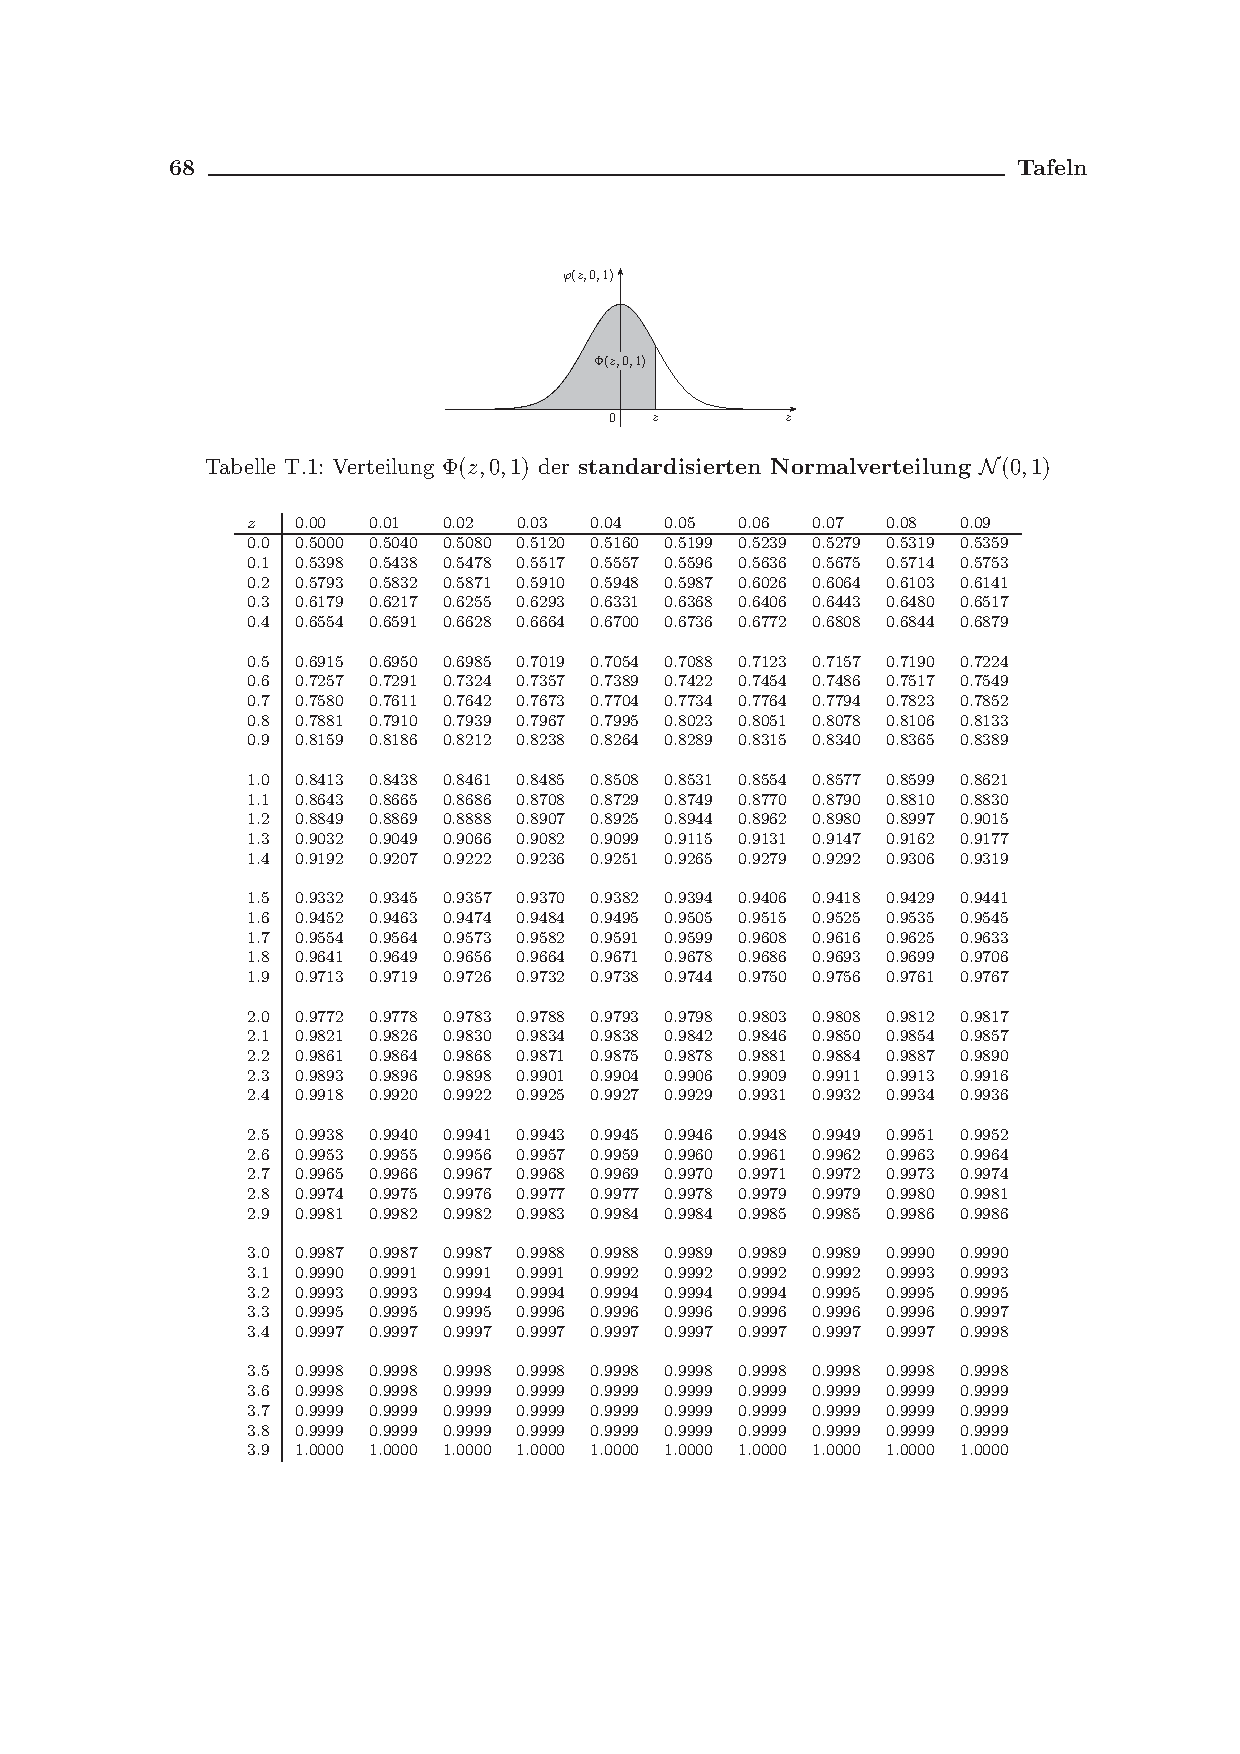
\includepdf[pages=1, trim=30mm 30mm 30mm 50mm,clip, offset = 0mm -25mm, scale = 0.85]{./appendix/Wahrscheinlichkeitstafeln.pdf}
\end{minipage}
\newpage

\subsection{Tafel: q-Quantile standardisierten Normalverteilung \cite{C:LookUpTable}}
\begin{minipage}{0.9\linewidth}	
	\label{Anh:TafelqQuantileStandardisierteNormalverteilung}
	\includepdf[pages=2, trim=25mm 30mm 25mm 35mm,clip, offset = 0mm -5mm, scale = 0.85]{./appendix/Wahrscheinlichkeitstafeln.pdf}
\end{minipage}
\newpage

\subsection{Tafel: Student-t-Verteilung \cite{C:LookUpTable}}
\begin{minipage}{0.9\linewidth}
	\label{Anh:TafelStudentTVerteilung}
	\includepdf[pages=3, trim=25mm 30mm 25mm 35mm,clip, offset = 0mm -5mm, scale = 0.85]{./appendix/Wahrscheinlichkeitstafeln.pdf}
\end{minipage}
\newpage

\subsection{Tafel: Faktoren für Konstruktion Kontrollkarten \cite{C:KonstruktionKontrollkarte}}
\begin{minipage}{0.9\linewidth}
	\label{Anh:TafelFaktorenKontrollkarten}
	\includepdf[pages=4, trim=25mm 30mm 25mm 35mm,clip, offset = 0mm -5mm, scale = 0.85]{./appendix/Wahrscheinlichkeitstafeln.pdf}
\end{minipage}
\newpage

\subsection{Tafel: Wichtigste Werte für $\sigma$}
\label{Anh:WichtigeSigma}
\begin{minipage}{\linewidth}
\begin{center}
		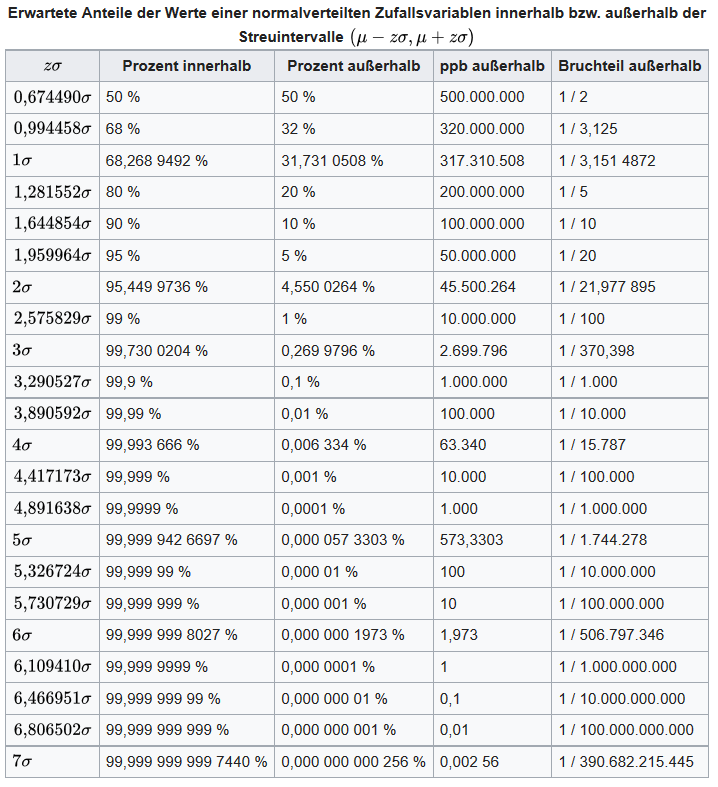
\includegraphics[width=0.8\linewidth]{figures/WichtigsteWerteSigma.png}\\
		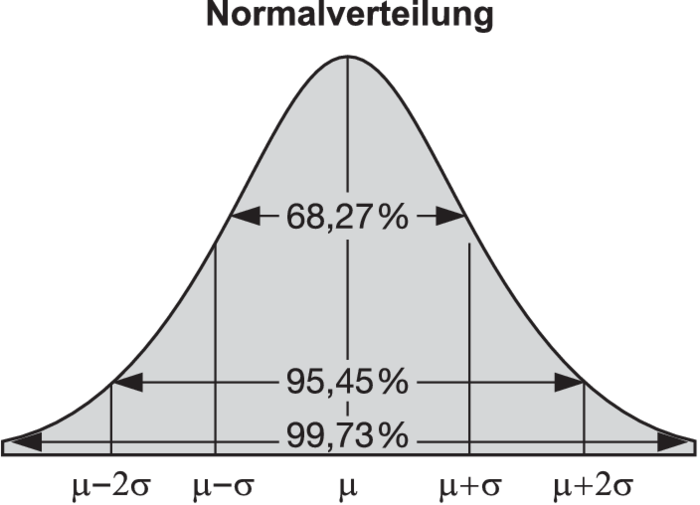
\includegraphics[width=0.3\linewidth]{figures/Normalverteilung.png}\\
		\textit{Quelle:}\cite{C:Normalverteilung}
\end{center}		

\end{minipage}
